% ===== Expanded figures/tables generated from frozen SEALED_TEST items =====
% (gen_figures.py + gen_expanded.py + gen_tables.py; no hand-typed numbers)

\subsection{Per-Arm Distribution Detail (RQ1/RQ2 supporting)}
The three arms differ little in central tendency but show distinct cost
distributions. Figure~\ref{fig:em_overall} restates end-to-end EM across arms;
Figures~\ref{fig:retr_dist}--\ref{fig:em_dist} show the full per-question
distributions of retrieval calls, LLM calls, latency, and EM, confirming that
the arms cluster near-identical medians while the chain arm's LLM-call tail is
heavier on HotpotQA (the source of its $+24$ LLM calls/question mean gap).
Figure~\ref{fig:evrecall} reports evidence recall, where the arms are again
near-identical.

\begin{figure}[t]
\centering
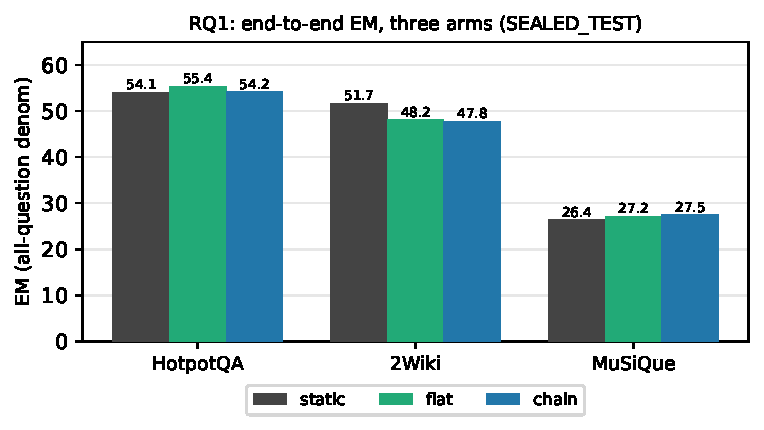
\includegraphics[width=0.62\columnwidth]{figures/fig1_em_overall.pdf}
\caption{RQ1: end-to-end EM under the all-question denominator, three arms.}
\label{fig:em_overall}
\end{figure}

\begin{figure}[t]
\centering
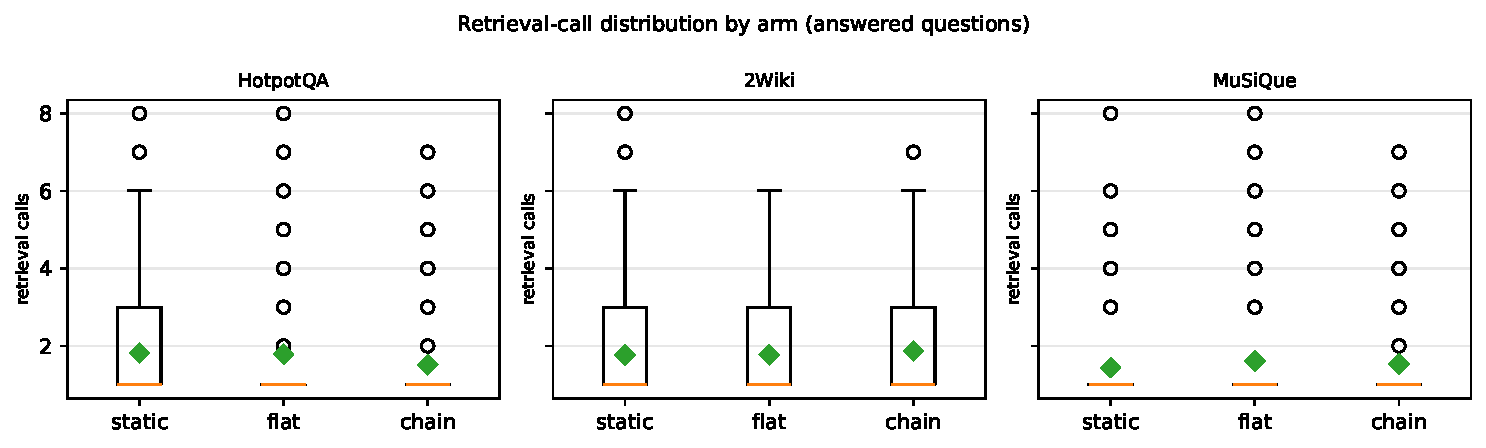
\includegraphics[width=0.92\columnwidth]{figures/fig_a_retr_dist.pdf}
\caption{RQ1/RQ2: retrieval-call distribution by arm (answered questions).
Medians are near-identical; the arms do not separate on retrieval cost.}
\label{fig:retr_dist}
\end{figure}

\begin{figure}[t]
\centering
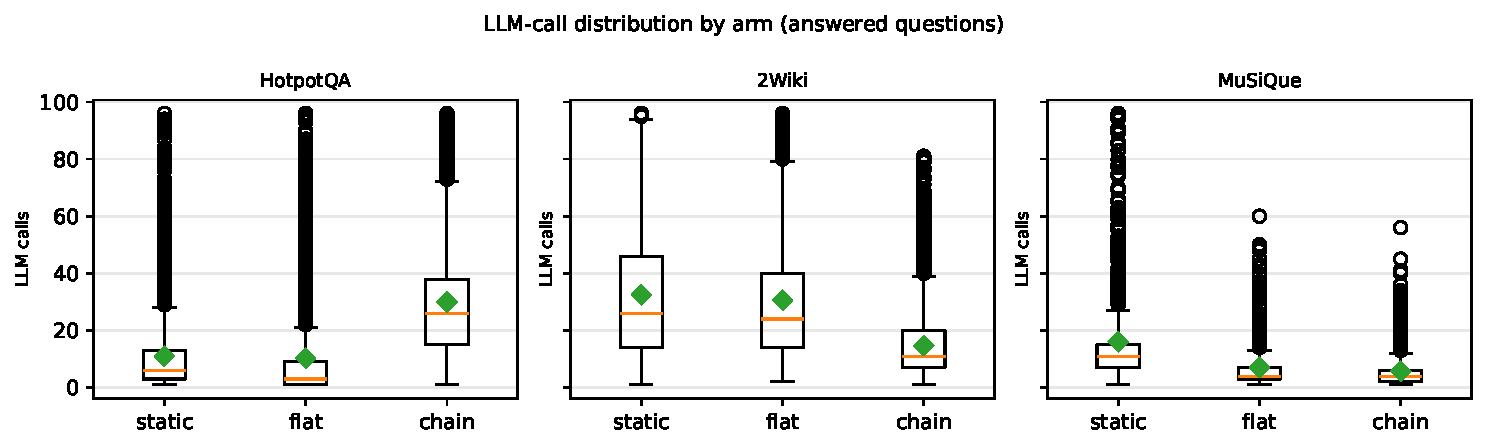
\includegraphics[width=0.92\columnwidth]{figures/fig_b_llm_dist.pdf}
\caption{RQ2: LLM-call distribution by arm. The chain arm's upper tail is
heavier on HotpotQA (more deep-exploration calls).}
\label{fig:llm_dist}
\end{figure}

\begin{figure}[t]
\centering
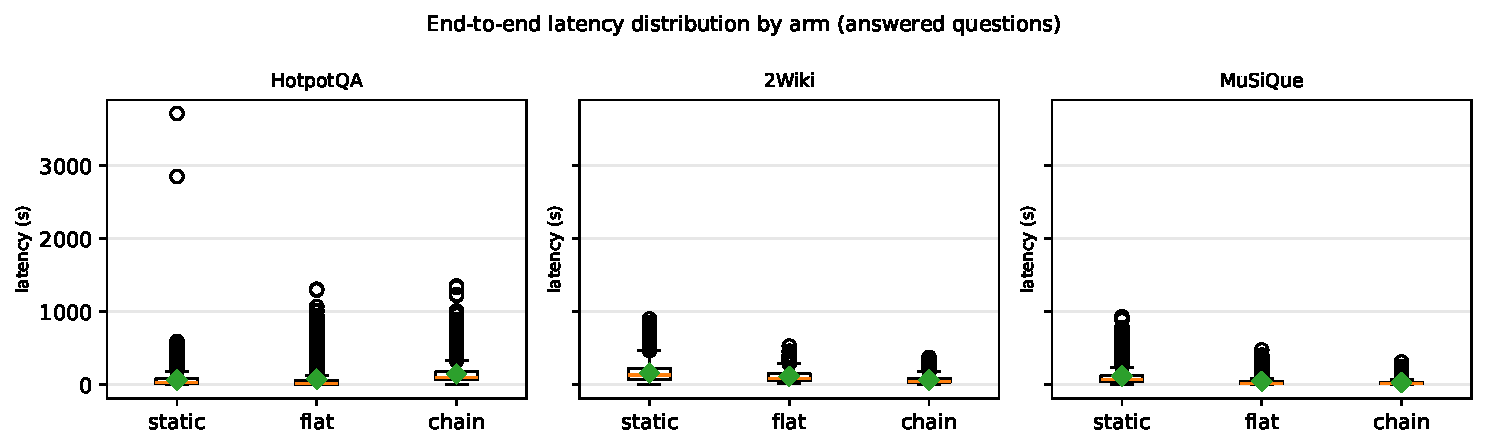
\includegraphics[width=0.92\columnwidth]{figures/fig_c_latency_dist.pdf}
\caption{RQ2: end-to-end latency distribution by arm.}
\label{fig:latency_dist}
\end{figure}

\begin{figure}[t]
\centering
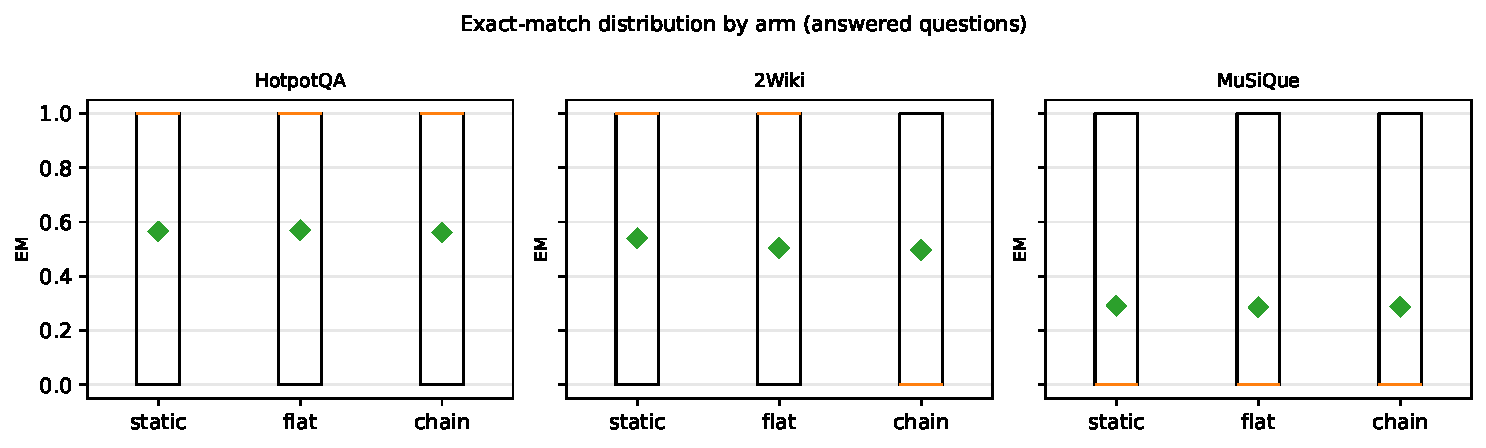
\includegraphics[width=0.92\columnwidth]{figures/fig_d_em_dist.pdf}
\caption{RQ1: exact-match distribution by arm (answered questions).}
\label{fig:em_dist}
\end{figure}

\begin{figure}[t]
\centering
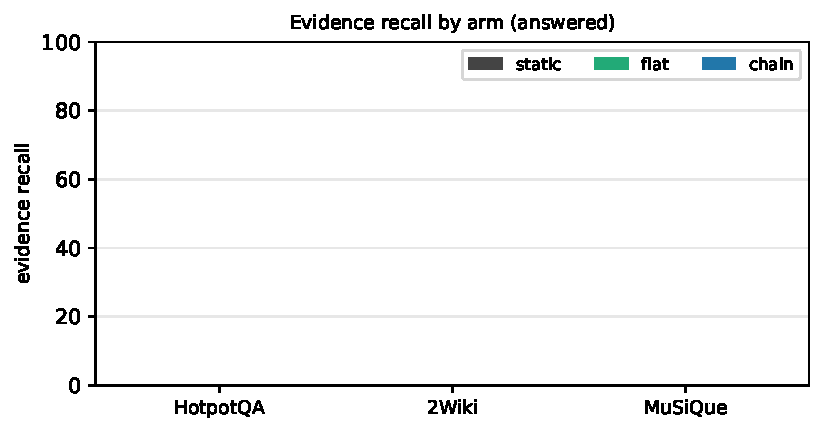
\includegraphics[width=0.55\columnwidth]{figures/fig_e_evrecall.pdf}
\caption{RQ1/RQ2: evidence recall by arm (answered questions).}
\label{fig:evrecall}
\end{figure}

\begin{figure}[t]
\centering
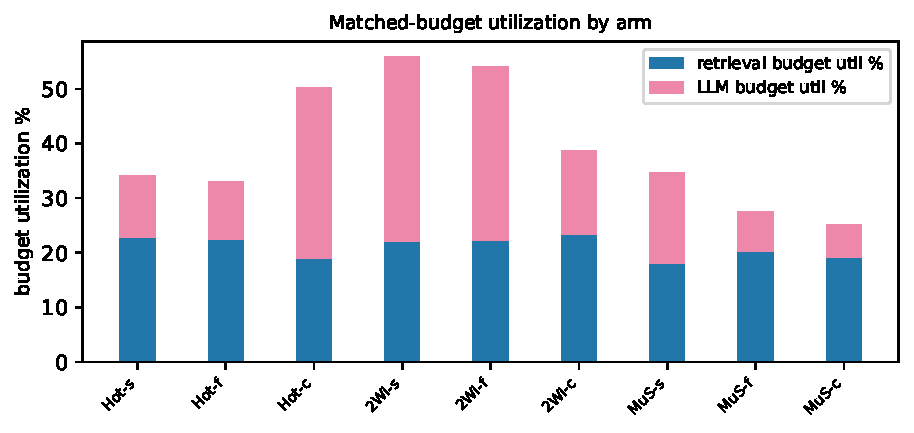
\includegraphics[width=0.72\columnwidth]{figures/fig_f_budget_util.pdf}
\caption{RQ2: matched-budget utilization (retrieval + LLM) by arm. The chain
arm consumes a larger share of its LLM budget on HotpotQA.}
\label{fig:budget_util}
\end{figure}

\begin{figure}[t]
\centering
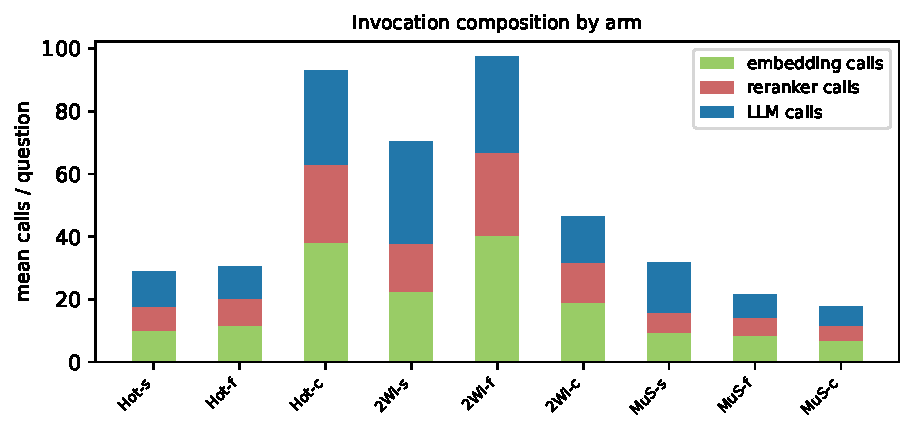
\includegraphics[width=0.72\columnwidth]{figures/fig_g_cost_comp.pdf}
\caption{RQ2: invocation composition (embedding / reranker / LLM calls) by arm.
The chain arm's extra LLM calls dominate its cost on HotpotQA.}
\label{fig:cost_comp}
\end{figure}

\subsection{Full Descriptive Statistics (supporting)}
Table~\ref{tab:descriptive} gives the complete per-arm descriptive statistics
(mean, median, p90, budget utilization, plan complexity, and invocation
counts) over the frozen SEALED\_TEST items; the numbers are machine-derived
from the run artifacts and are not hand-edited. Table~\ref{tab:paired_full}
gives the full paired chain-vs-static differences (EM, retrieval, LLM,
documents, latency) with bootstrap 95\% confidence intervals on shared
questions. Table~\ref{tab:failure_arm} breaks the execution status down by
arm and dataset, and Table~\ref{tab:evidence} reports the evidence-quality
metrics (recall, MRR, retrieved documents) by arm.

\begin{table}[t]
\centering
\caption{Full per-arm descriptive statistics on SEALED\_TEST (machine-derived
from run items; source \code{tableA\_descriptive.csv}).}
\label{tab:descriptive}
\scriptsize
\makeatletter
\begin{tabular}{llrrrrrrrrrrrr}
\toprule
dataset & arm & n & ok & budg & EM & F1 & evRec & retr & LLM & docs & lat(s) & retrU\% \\
\midrule
\@@input tables/tabA_body.tex
\bottomrule
\end{tabular}\makeatother

\end{table}

\begin{table}[t]
\centering
\caption{Paired chain-vs-static differences on shared questions, bootstrap 95\%
CI (seed 2027). Source \code{tableB\_paired.csv}.}
\label{tab:paired_full}
\scriptsize
\makeatletter
\begin{tabular}{llrrrrrr}
\toprule
dataset & metric & chain & static & $\Delta$ & CI$_{2.5}$ & CI$_{97.5}$ & n \\
\midrule
\@@input tables/tabB_body.tex
\bottomrule
\end{tabular}\makeatother

\end{table}

\begin{table}[t]
\centering
\caption{Execution status by arm $\times$ dataset (source
\code{tableC\_failure\_by\_arm.csv}).}
\label{tab:failure_arm}
\scriptsize
\makeatletter
\begin{tabular}{llrrrrrr}
\toprule
dataset & arm & ok & budget & boundary & other & total & ok\% \\
\midrule
\@@input tables/tabC_body.tex
\bottomrule
\end{tabular}\makeatother

\end{table}

\begin{table}[t]
\centering
\caption{Evidence-quality metrics by arm (source \code{tableD\_evidence.csv}).}
\label{tab:evidence}
\scriptsize
\makeatletter
\begin{tabular}{llrrrr}
\toprule
dataset & arm & evRecall & evRecall(med) & evMRR & docs \\
\midrule
\@@input tables/tabD_body.tex
\bottomrule
\end{tabular}\makeatother

\end{table}
